%Chapter 6

\renewcommand{\thechapter}{6}

\chapter{Adaptive Consistency}
\label{ch:adaptive_consistency}

Throughout this dissertation we've outlined a planetary-scale data storage system composed of a two-tier structure that provides a hybrid consistency model.
Both tiers are designed to scale to thousands of replicas, and together could represent millions of replicas operating in concert around the world.
Management and systems administration of such a large scale system using external monitoring processes is impractical at best and prohibitively complex at worse.
Even with a trusted infrastructure of cloud services, building a single synchronization point for monitoring and optimization would require the online collection of live information from across the globe, which itself would be susceptible to delays and partitions of the kind the administrator would be trying to manage.
Even if those delays could be managed, such a synchronization point would have to manage a huge number of events streaming in from a large number of sources, which has challenges in and of itself~\cite{spark_streaming}.

Instead, we propose that an \emph{emergent model} of network behavior is required to tune and optimize planetary scale systems in an online fashion such that local, simple rules lead to globally emergent behavior~\cite{bengfort_evolutionary_2014}.
Specifically we hypothesize that when individual replicas follow simple optimization procedures based on monitoring of their local network performance, access patterns, queries to their neighbors, and other environmental factors the performance of the system will collectively increase.
Because we focus primarily on the consistency aspects of geo-replicated data storage, we have termed this behavior \emph{adaptive consistency}, because with a hybrid or continuous consistency model, such optimizations will minimize inconsistent behaviors due to latency or configuration.

Although this work is largely left for future research on a fully deployed platform, we have built our system with this kind of adaptation in mind.
To validate our thought process, we have conducted an experiment that primarily adapts the federated fog layer of our system by modifying anti-entropy selection with reinforcement learning techniques~\cite{bengfort_anti-entropy_2018}.
In this chapter we will show we can improve consistency of the system as a whole with localized machine learning implemented on a per-replica basis.
We will then finish with a discussion of how we can generalize this process to other techniques in the system as a whole.

\section{Anti-Entropy Bandits}

A distributed system is made highly available when individual servers are
allowed to operate independently without failure-prone, high latency
coordination.
The independent nature of the server's behavior means that it can immediately
respond to client requests, but that it does so from a limited, local
perspective which may be inconsistent with another server's response.
If individual servers in a system were allowed to remain wholly independent,
individual requests from clients to different servers would create a lack of
order or predictability, a gradual decline into inconsistency, i.e. the
system would experience \textit{entropy}.
To combat the effect of entropy while still remaining highly available,
servers engage in periodic background \textit{anti-entropy
  sessions}~\cite{bayou}.

Anti-entropy sessions synchronize the state between servers ensuring that,
at least briefly, the local state is consistent with a portion of the global
state of the system.
If all servers engage in anti-entropy sessions, the system is able to make
some reasonable guarantees about consistent replication; the most famous
of which is that without requests the system will become
globally consistent, eventually~\cite{anti_entropy}.
More specifically, inconsistencies in the form of stale reads can be bound by
likelihoods that are informed by the latency of anti-entropy sessions and the
size of the system~\cite{probabilistically_bounded_staleness,quantifying_pbs}.
Said another way, overall consistency is improved in an eventually consistent
system by decreasing the likelihood of a stale read, which is tuned by
improving the \textit{visibility latency} of a write, the speed at which a
write is propagated to a significant portion of servers.
This idea has led many system designers to decide that eventual consistency
is ``consistent enough''~\cite{bermbach_eventual_2011,wada_data_2011},
particularly in a data center context where visibility latency is far below
the rate of client requests, leading to practically strong consistency.

However, propagation rates need to be re-evaluated when replicas move outside of data center contexts and when anti-entropy is replicating across the wide area.
Our system envisions a fog layer that provides data services to localized regions with a hybrid consistency model.
The edge is specifically designed to handle mobile users, sensor systems, and high throughput applications the edge of the data center backbone~\cite{edge_computing,geo_cdn}.
However, scaling an eventually consistent system to dozens or even hundreds
of nodes increases the radius of the network, which leads to increased noise
during anti-entropy e.g. the possibility that an anti-entropy session will be
between two already synchronized nodes.
Geographic distribution and extra-datacenter networks also increase the
latency of anti-entropy sessions so that inconsistencies become more apparent
to external observers.

To address this challenge, we propose the use of reinforcement learning techniques to optimize network behavior to minimize latency.
Anti-entropy uses gossip and rumor spreading to propagate updates
deterministically without saturating the
network even in the face of network
outages~\cite{gossip_protocols,rumor_spreading,rumor_spreading_dynamics}.
These protocols use uniform random selection to choose synchronization peers,
which means that a write occurring at one replica is not efficiently
propagated across the network.
In this section we explore the use of \textit{multi-armed bandit}
algorithms~\cite{epoch_greedy_mab,contextual_bandits} to optimize
for fast, successful synchronizations by modifying peer selection
probabilities.
The result is a synchronization topology that emerges according to access
patterns and network latencies.
Such topologies produce efficient synchronization,
localize most data exchanges, lower visibility latency, and increase
consistency.

\subsection{Accesses and Consistency}

In this section we review the access and consistency model in the context of bandits as well as how anti-entropy is conducted.
A more complete discussion of these topics can be found in Chapter~\ref{ch:federated_consistency}.

Clients can \texttt{Put} (write) and \texttt{Get} (read) key-value pairs to
and from one or more replicas in a single operation, creating read and write quorums that improve consistency by enforcing coordination between replicas on the access.
In large, geo-replicated systems, we assume that clients prefer to choose fewer, local replicas to connect with, assuming that writes are primarily local and reads are global.
On \texttt{Put}, a new conflict-free version of the write is created.
This results in the possibility of two types of inconsistencies that occur during concurrent accesses: stale reads and forked writes.
As a write is propagated through the system, the latest-writer wins policy means that at least one of the forks will be ``stomped'', e.g. not fully replicated.

Both forms of inconsistency can be primarily attributed to \emph{visibility
latency}, that is the time it takes for an update to propagate to all
replicas in the system.
Visibility latency is directly related to the likelihood of stale reads with
respect to the frequency of accesses~\cite{quantifying_pbs}; said
another way, decreasing the visibility latency improves the overall
consistency of a system.
However, in a system that uses anti-entropy for replication, the propagation
speed of an update is not governed solely by network connections, it is also
bound to the number and frequency of anti-entropy sessions conducted as well
as the radius of the network.

Visibility latency is minimized when all replicas choose a remote
synchronization partner that does not yet have the update.
This means that minimal visibility latency is equal to $t\log_3n$, where
$t$ is the anti-entropy interval and $n$ is the number of replicas in the
network.
In practice, however, because of inefficient exchanges due to uniform random
selection of synchronization partners, this latency is never practically
achieved, and is instead modulated by a noise variable that is
proportional to the size of the network.

\subsection{Multi-Armed Bandits}

To combat the effect of noise on visibility latency our initial approach
employs a technique commonly used in active and reinforcement learning:
multi-armed bandits.
Multi-armed bandits refer to a statistical optimization procedure that is
designed to find the optimal payout of several choices that each have
different probabilities of reward.
In this case, we use bandits to improve uniform random selection of peers so
that replicas choose synchronization partners that are most likely to exchange
information, and thus more quickly propagate updates, while still maintaining
the properties of full replication and fault tolerance.

A bandit problem is designed by identifying several (usually more than two)
competing choices called ``arms''\renewcommand{\baselinestretch}{1} \small\footnotesize\footnote{Arms refer to the pulling
mechanism of a slot machine, the metaphor generally used to motivate the
multi-armed bandit problem.}\renewcommand{\baselinestretch}{2} \small\normalsize, as well as a reward function that determines how
successful the selection of an arm is.
During operation, the bandit selects an arm, observes the rewards, then
updates the payout likelihood of the selected arm, normalized by the number
of selections.
As the bandit selects arms, it learns which arm or arms have the highest
likelihood of reward, and can modify it's arm selection \emph{strategy} to
maximize the total reward over time.

Bandits must balance exploration of new arms with possibly better reward
values and exploitation of an arm that has higher rewards than the other.
In the \emph{epsilon greedy strategy}, the bandit will select the arm with
the best reward with some probability $1-\epsilon$, otherwise it will select
any of the arms with uniform probability.
The smaller $\epsilon$ is, the more the bandit favors exploitation of known
good arms, the larger $\epsilon$ is, the more it favors exploration.
If $\epsilon=1$ then the algorithm is simply uniform random selection.
A simple extension of this is a strategy called \emph{annealing epsilon
greedy}, which starts with a large $\epsilon$, then as the number of trials
increases, steadily decreases $\epsilon$ on a logarithmic scale.
There are many other bandit strategies but we have chosen these two simple
strategies for our initial research to demonstrate a bolt-on effective
improvement to existing systems.

Peer selection for anti-entropy is usually conducted with uniform random
selection to guarantee complete replication.
To extend anti-entropy with bandits, we design a selection method whose arms
are remote peers and whose rewards are determined by the success of
synchronization.
The goal of adding bandits to anti-entropy is to optimize selection of peers
such that the visibility latency becomes closer to the optimal propagation
time as a synchronization topology emerges from the bandits.
A secondary goal is to minimize anti-entropy latency by preferring local (in
the same data center) and regional (e.g. on the same continent) connections.

Our initial reward function favors synchronizations to replicas where the
most writes are occurring by giving higher rewards to anti-entropy sessions
that exchange later versions in either a push or a pull, as well as additional
rewards if more than one object is exchanged.
Additionally, the latency of the synchronization RPCs is computed to reward
replicas that are near each other.
The complete reward function is given in Table~\ref{tab:ch06_rewards}: for each
phase of synchronization (push and pull), compute the reward as the sum of the
propositions given.
For example if a synchronization results in three objects being pulled in
250ms, and one object being pushed in 250ms, the reward is 0.75.

\renewcommand{\baselinestretch}{1}
\small\normalsize
 \begin{table}[ht]
\caption[Bandit Reward Function]{The rewards function for our initial anti-entropy bandits. Rewards are computed by introspecting the results of the pull and push phases of bilateral anti-entropy.}
\begin{center}
\begin{tabular}{@{}l c c c @{}}
\hline
& \textbf{Pull} & \textbf{Push} & \textbf{Total} \\
\hline \hline
Synchronize at least 1 object & 0.25 & 0.25 & 0.50 \\
Additional for multiple objects  & 0.05 & 0.05 & 0.10 \\
Latency $\leq$ 5ms (local)        & 0.10 & 0.10 & 0.20 \\
Latency $\leq$ 100ms (regional)   & 0.10 & 0.10 & 0.20 \\
\hline
\textit{Total} & \textit{0.50} & \textit{0.50} & \textit{1.00} \\
\hline
\end{tabular}
\end{center}
\label{tab:ch06_rewards}
\end{table}
 \renewcommand{\baselinestretch}{2}
\small\normalsize

The design of reward functions can be implemented to the needs of a specific
system.
For example, in a system that has workloads with variable sized writes, object
size could be considered or systems with imbalanced deployments might
consider a reward function that prioritizes inter-region communication.

\subsection{Experiments}

We conducted experiments using a distributed key-value store totally
replicated across 45 replicas in 15 geographic regions on 5 continents
around the world.
Replicas were hosted using AWS EC2 t2.micro instances and were connected to
each other via internal VPCs when in the same region, using external
connections between regions.
The store, called Honu, is implemented in Go 1.9 using gRPC and protocol
buffers for RPC requests; all code is open source and available on GitHub.

\begin{figure}
    \begin{center}
        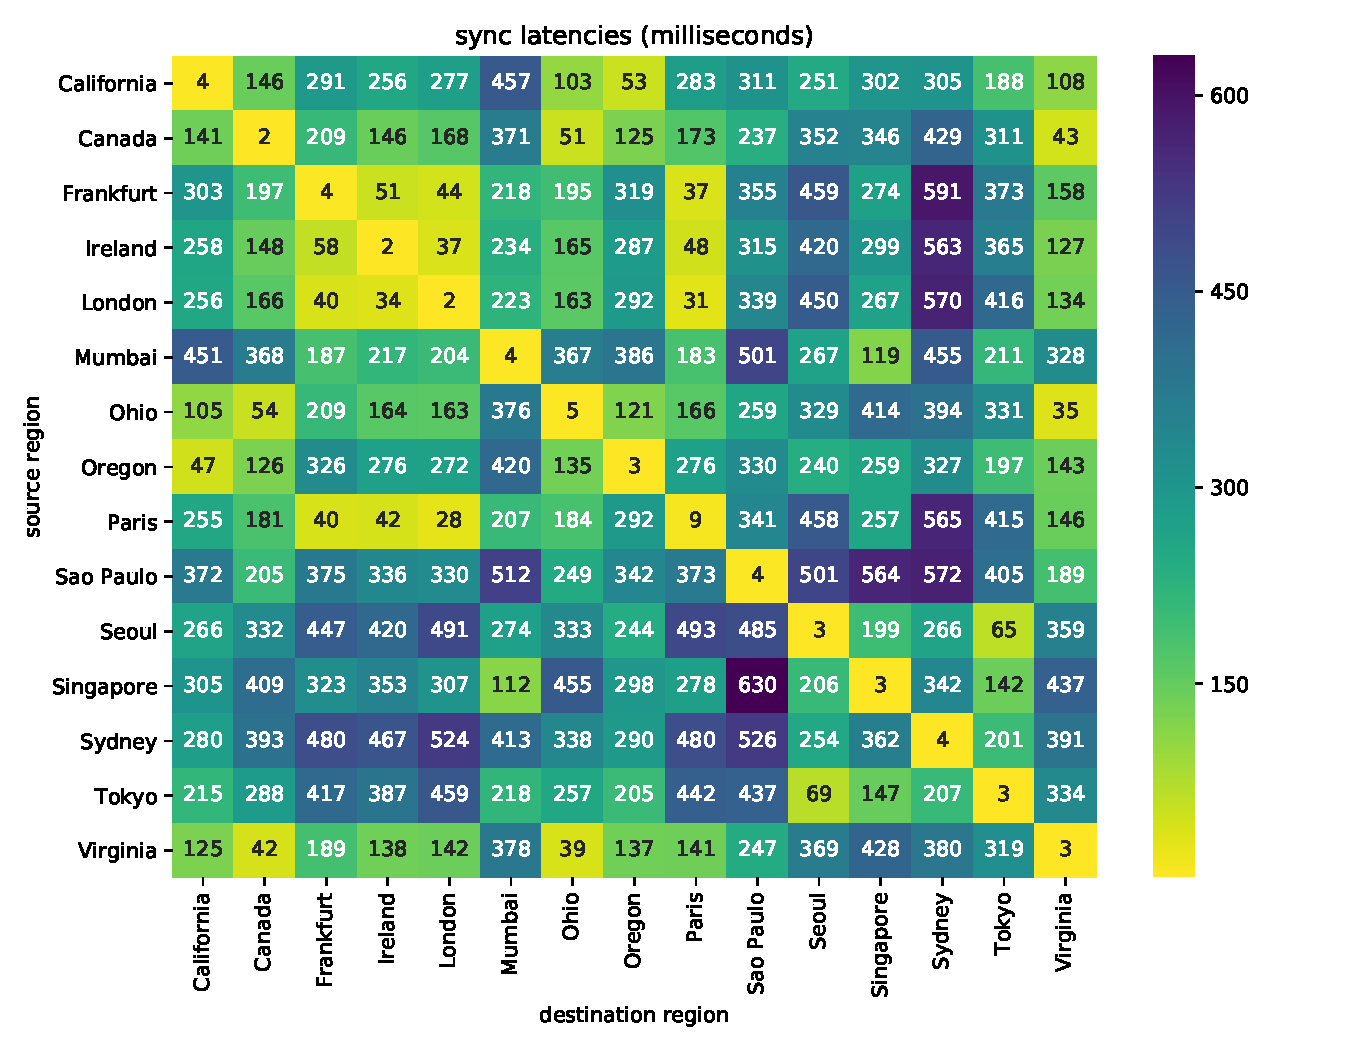
\includegraphics[width=5in]{figures/ch06_latency_sync_heatmap.pdf}
    \end{center}
    \renewcommand{\baselinestretch}{1}
    \small\normalsize

    \begin{quote}
        \caption[Anti-Entropy Synchronization Latencies]{Inter-Region Synchronization Latencies (Push+Pull)}
        \label{fig:ch06_latency_sync_heatmap}
    \end{quote}
\end{figure}
\renewcommand{\baselinestretch}{2}
\small\normalsize

\begin{figure}
    \begin{center}
        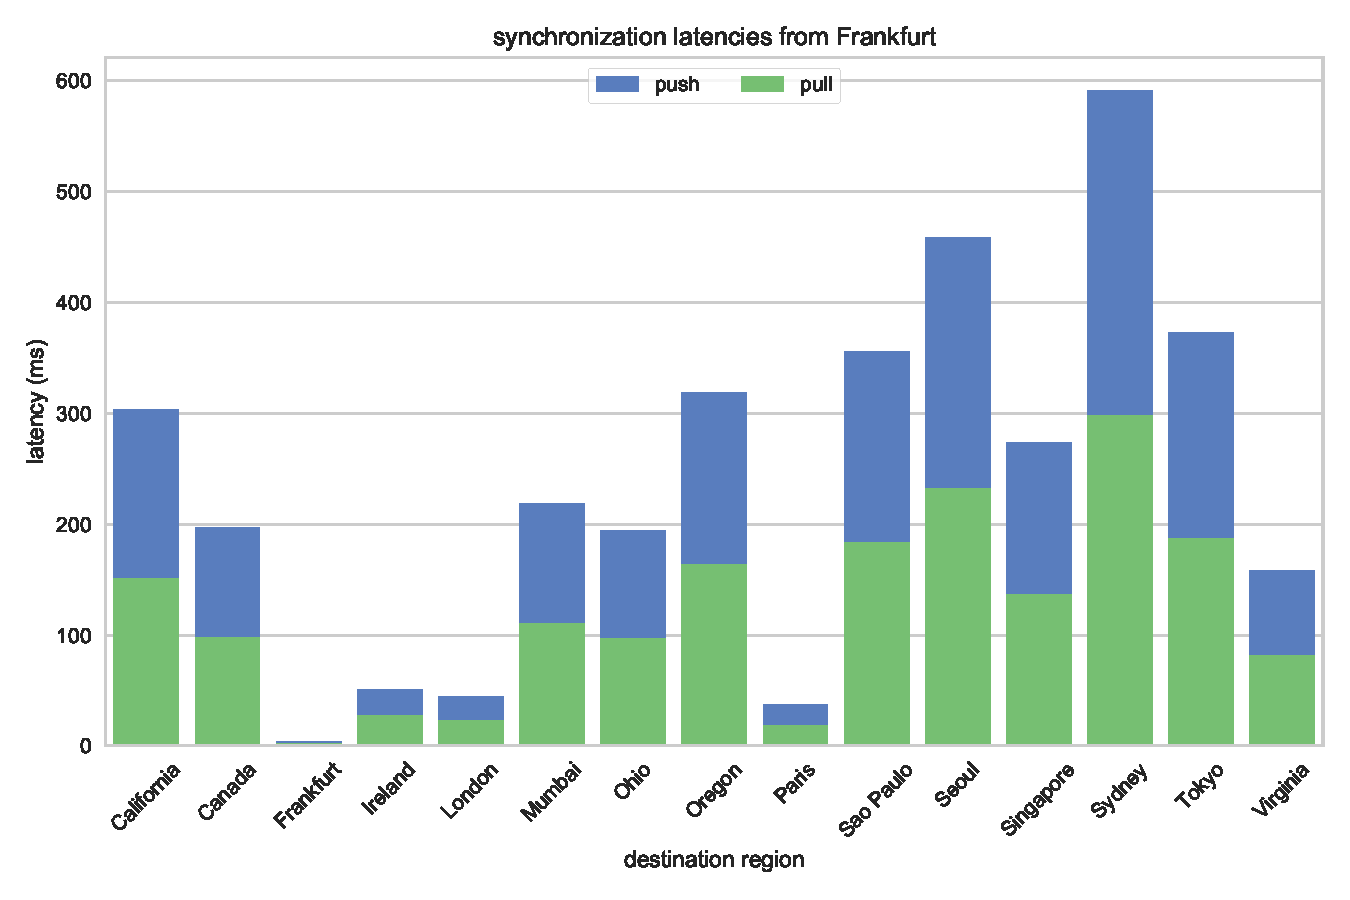
\includegraphics[width=5in]{figures/ch06_push_pull_frankfurt_latencies.pdf}
    \end{center}
    \renewcommand{\baselinestretch}{1}
    \small\normalsize

    \begin{quote}
        \caption[Anti-Entropy Synchronization Latency from Frankfurt]{View of anti-entropy synchronization latency from Europe and corresponding network distances.}
        \label{fig:ch06_push_pull_frankfurt_latencies}
    \end{quote}
\end{figure}
\renewcommand{\baselinestretch}{2}
\small\normalsize

The workload on the system was generated by 15 clients, one in each region and
colocated with one of the replicas.
Clients continuously created Put requests for random keys with a unique
prefix per-region such that consistency conflicts only occur within a
single region.
The average throughput generated per-client was 5620.4 puts/second.
The mean synchronization latency between each region ranged from 35ms to
630ms as shown in Figures~\ref{fig:ch06_latency_sync_heatmap} and \ref{fig:ch06_push_pull_frankfurt_latencies}.
To ensure at least one synchronization per anti-entropy session, we set the
anti-entropy interval to 1 second to train the system, then reduced the
interval to 125ms while measuring visibility latency.
To account for lag between commands sent to replicas in different regions,
each experiment was run for 11 minutes, the bandit learning period was 4
minutes then visibility latency was observed for 6 minutes, buffered by 30
seconds before and after the workload to allow replicas to initialize and
gracefully shutdown.

\begin{figure}
    \begin{center}
        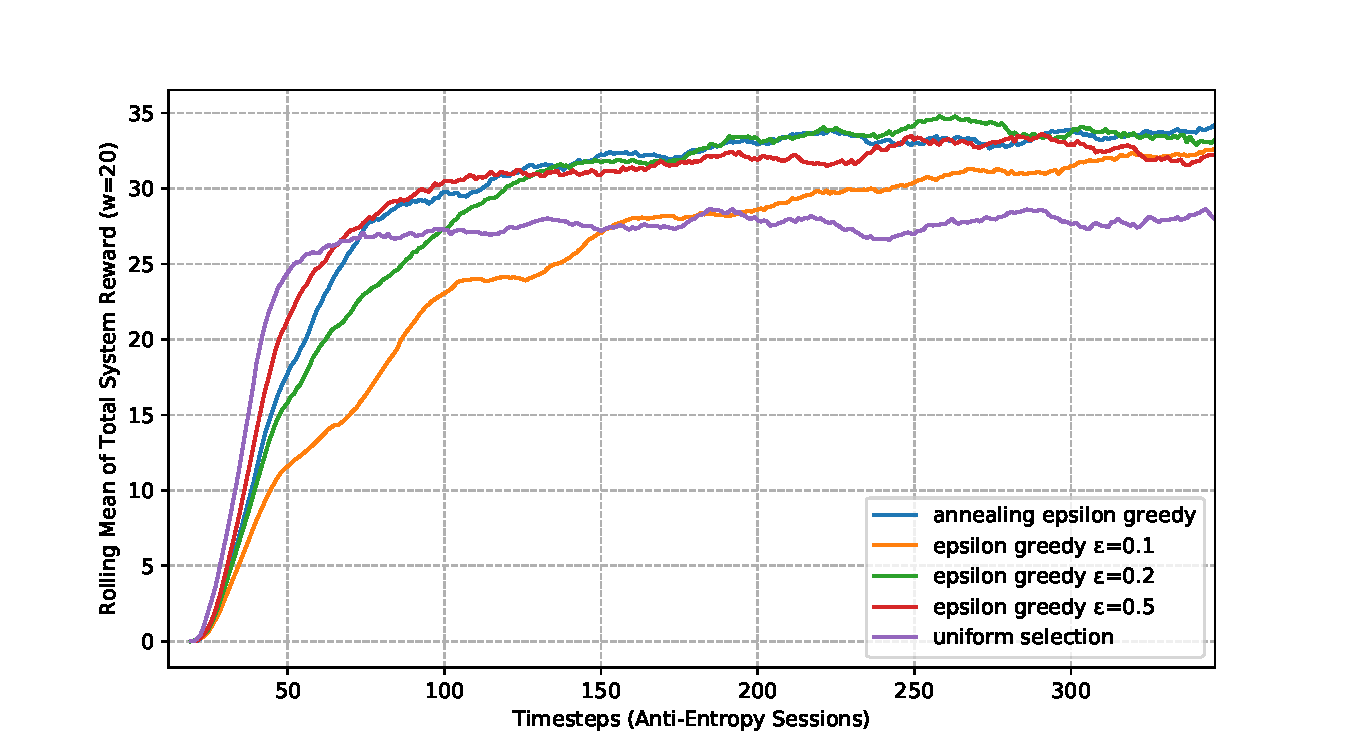
\includegraphics[width=5in]{figures/ch06_rewards.pdf}
    \end{center}
    \renewcommand{\baselinestretch}{1}
    \small\normalsize

    \begin{quote}
        \caption[Bandit Rewards]{Total system rewards over time.}
        \label{fig:ch06_rewards}
    \end{quote}
\end{figure}
\renewcommand{\baselinestretch}{2}
\small\normalsize

Our first experiments compared uniform random peer selection with epsilon
greedy bandits using $\epsilon \in \{0.1, 0.2, 0.5\}$ as well as an annealing
epsilon greedy bandit.
The total system rewards as a rolling mean over a time window of 20
synchronizations are shown in Figure~\ref{fig:ch06_rewards}.
The rewards ramp up from zero as the clients come online and start
creating work to be synchronized.
All of the bandit algorithms eventually improve over the baseline of uniform
selection, not only generating more total reward across the system, but also
introducing less variability in rewards over time.
None of the bandit curves immediately produces high rewards as they explore
the reward space; lower $\epsilon$ values may cause exploitation of incorrect
arms, while higher $\epsilon$ values take longer to find optimal topologies.
However, in the static workload case, the more aggressive bandit strategies
converge more quickly to the optimal reward.

\begin{figure}
    \begin{center}
        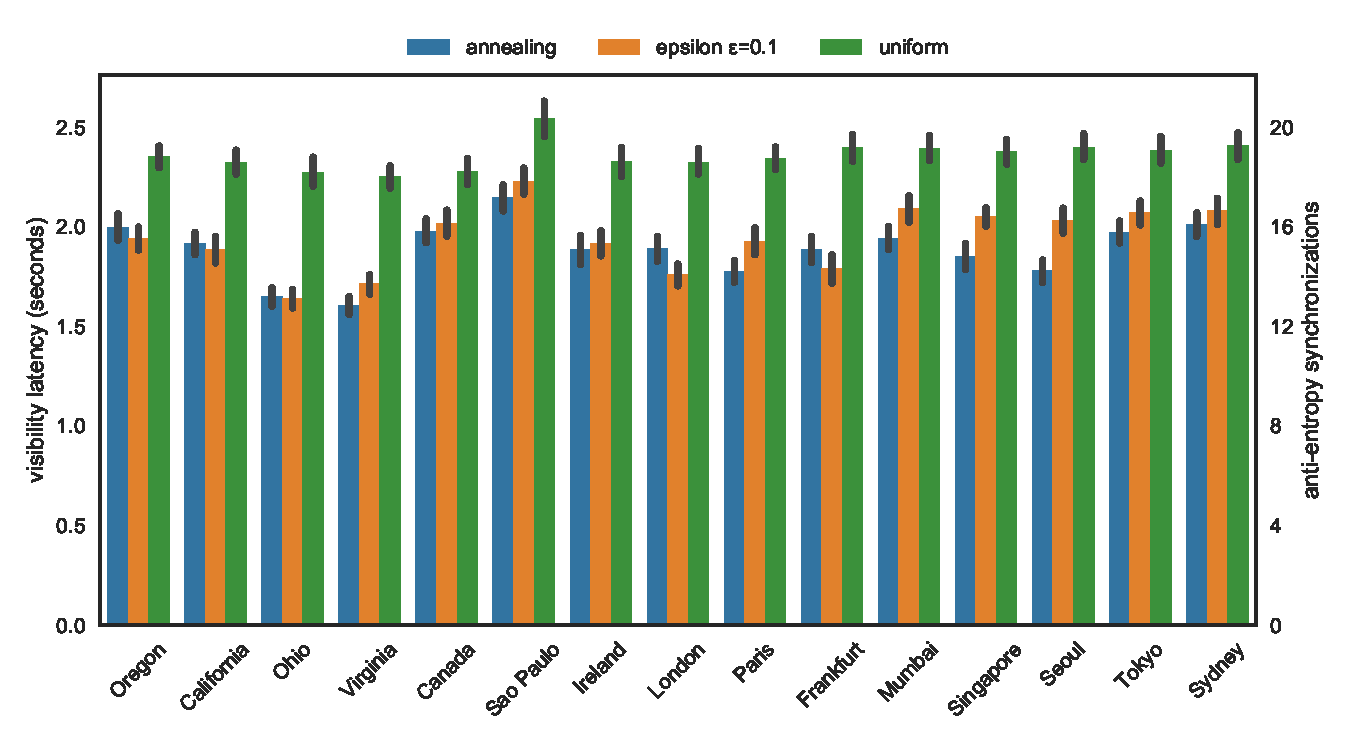
\includegraphics[width=5in]{figures/ch06_visibility_latency.pdf}
    \end{center}
    \renewcommand{\baselinestretch}{1}
    \small\normalsize

    \begin{quote}
        \caption[Visibility Latency]{Decreasing visibility latency from bandit approaches.}
        \label{fig:ch06_visibility_latency}
    \end{quote}
\end{figure}
\renewcommand{\baselinestretch}{2}
\small\normalsize

Visibility latencies were computed by reducing the workload rate to once
every 4 seconds to ensure the write becomes fully visible across the entire
network.
During the visibility measurement period, replicas locally logged the
timestamp the write was pushed or pulled; visibility latency is computed as
the difference between the minimum and maximum timestamp.
The average visibility latency per region is shown in
Figure~\ref{fig:ch06_visibility_latency} measured by the left y-axis.
Because the anti-entropy delay is a fixed interval, the estimated number of
required anti-entropy sessions associated with the visibility delay is shown
on the right y-axis of the same figure.
Employing bandit strategies reduces the visibility latency from 2360ms on
average in the uniform case to 1870ms, reducing the number of required
anti-entropy intervals by approximately 4.

To show the emergent behavior of bandits, we have visualized the resulting
topologies as network diagrams in Figure~\ref{fig:ch06_uniform_selection_topology} (uniform
selection), Figure~\ref{fig:ch06_annealing_epsilon_toplogy} (annealing epsilon) and
Figure~\ref{fig:ch06_epsilon_greedy_topology} (epsilon greedy $\epsilon=0.2$).
Each network diagram shows each replica as a vertex, colored by region e.g.
purple is California, teal is Sao Paulo, Brazil, etc.
Each vertex is also labeled with the 2-character UN country or US state
abbreviation as well as the replica's precedence id.
The size of the vertex represents the number of \texttt{Put} requests that
replica received over the course of the experiment; larger vertices
represent replicas that were colocated with workload generators.
Each edge between vertices represents the total number of successful
synchronizations, the darker and thicker the edge is, the more
synchronizations occurred between the two replicas.
Edges are directed, the source of the edge is the replica that initiated
anti-entropy with the target of the edge.

\begin{figure}
    \begin{center}
        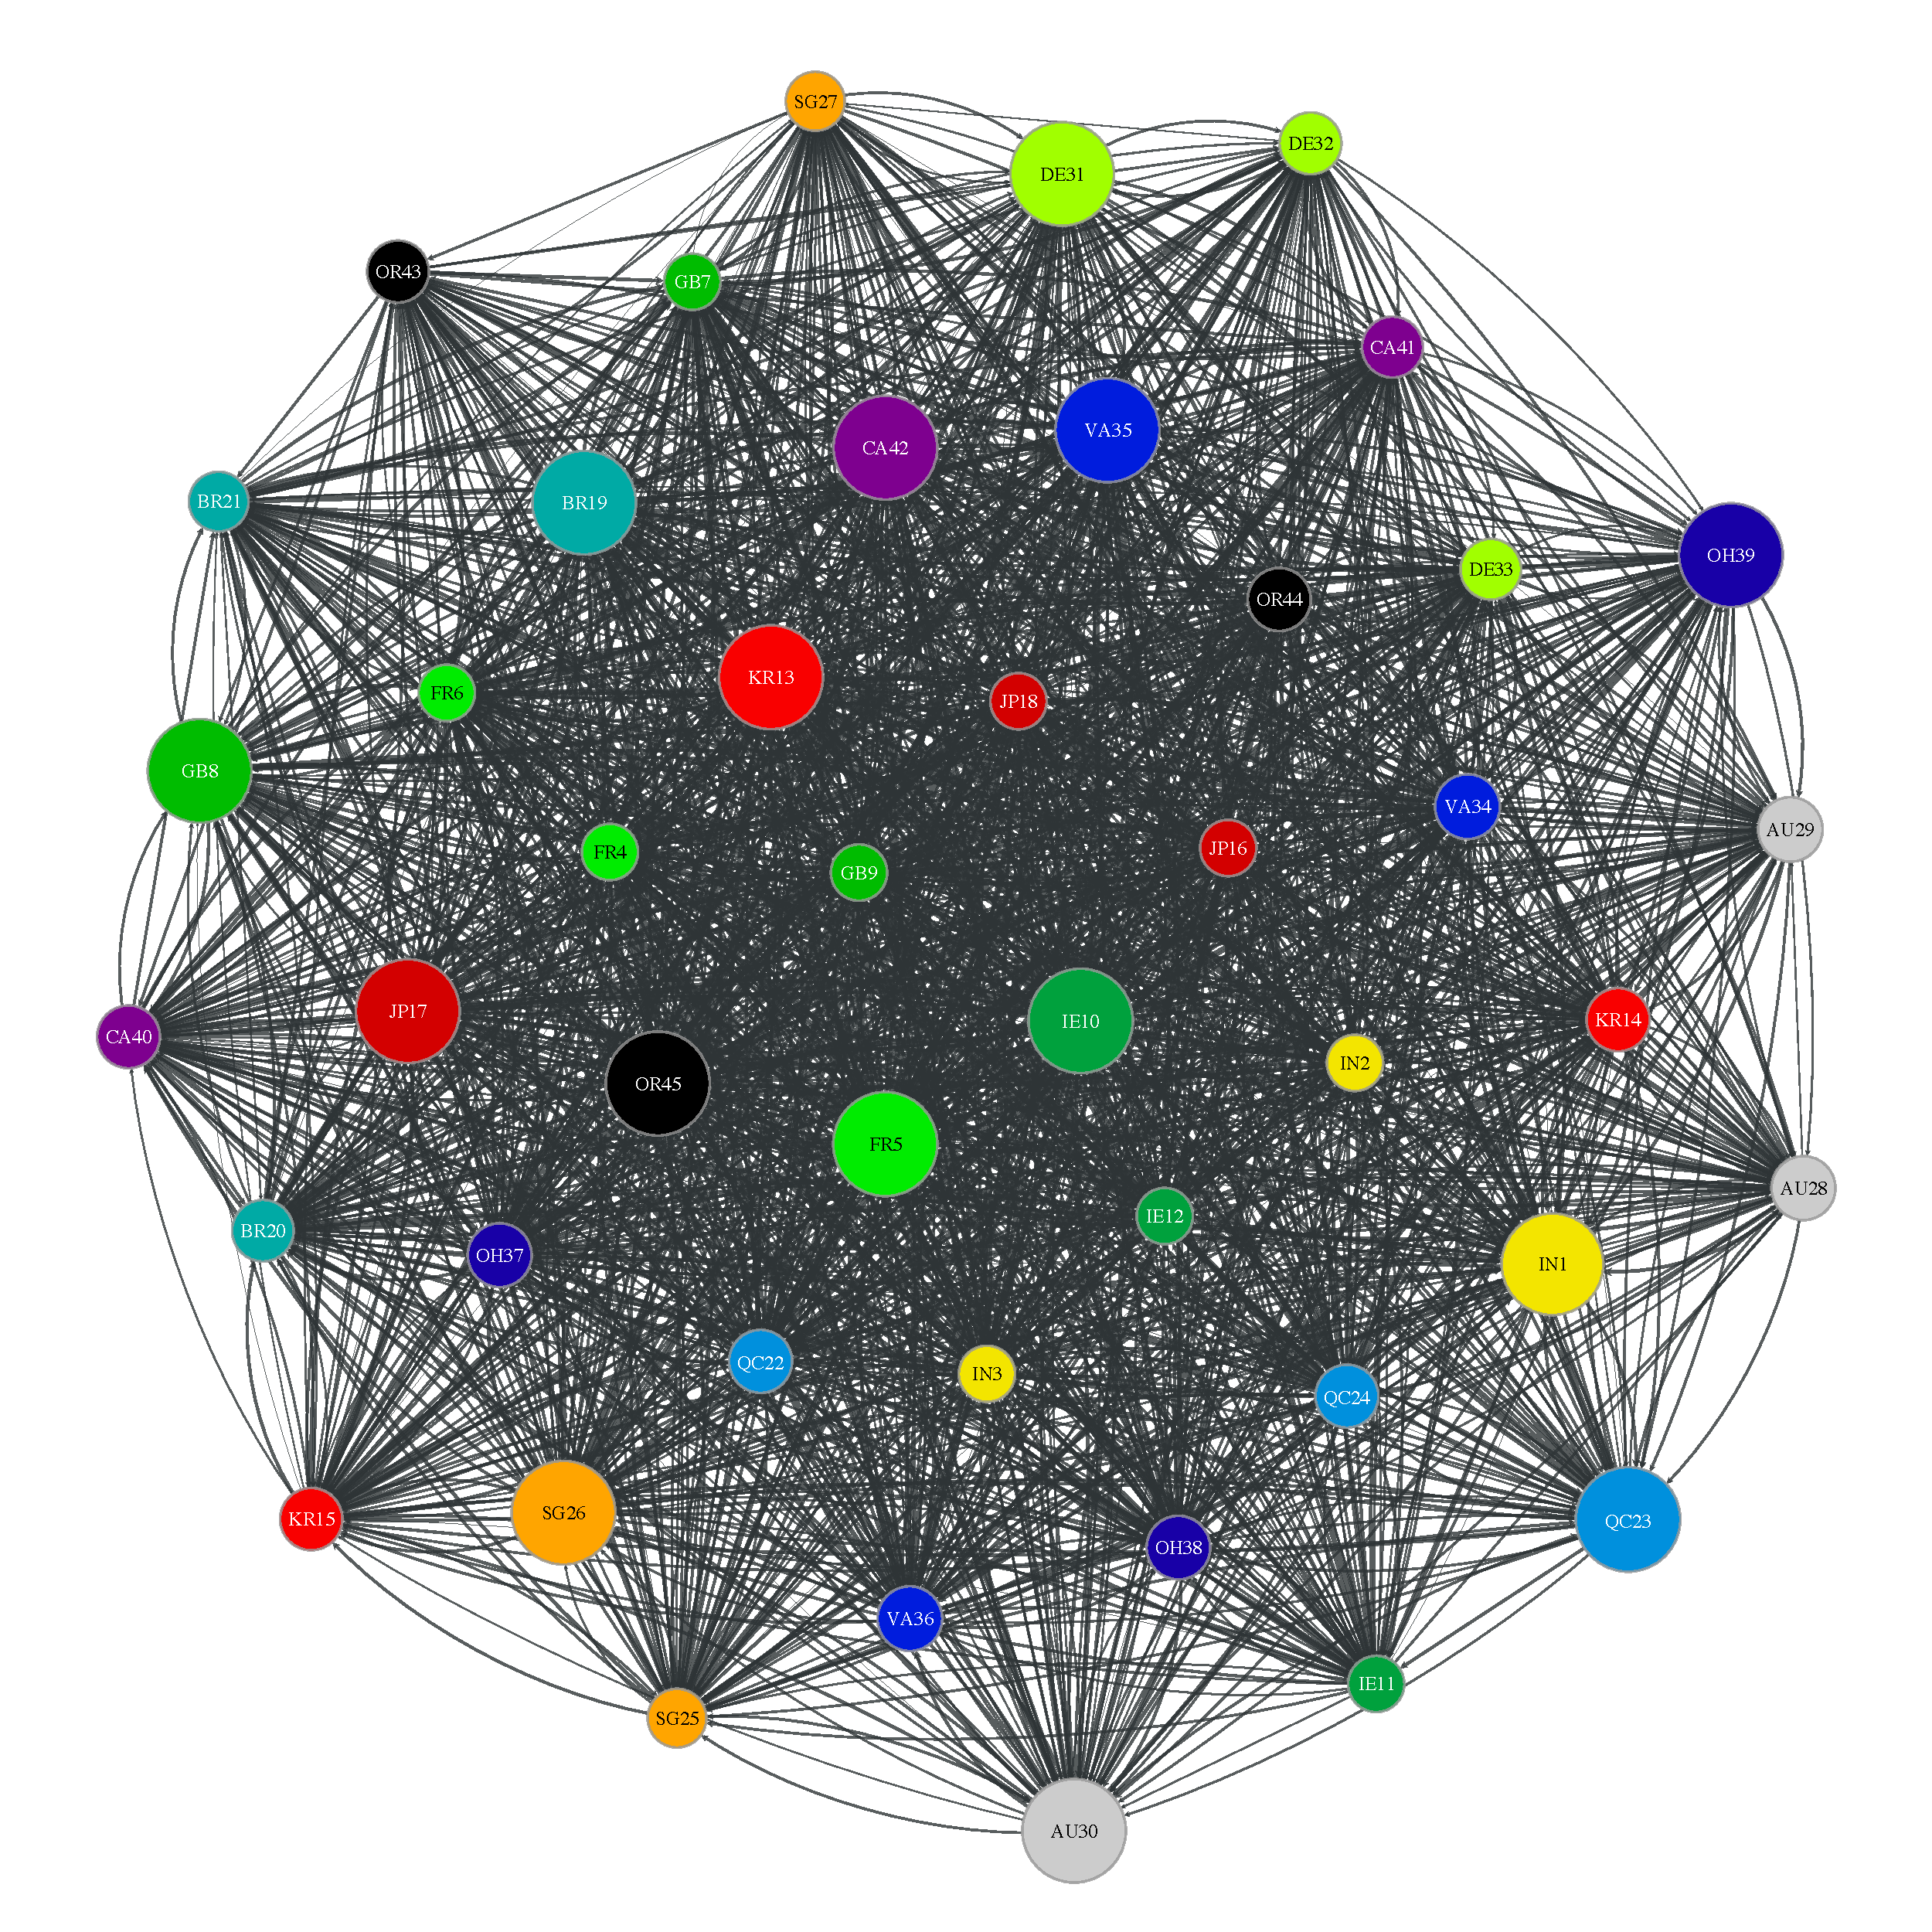
\includegraphics[width=5in]{figures/ch06_b-uniform-selection-e1.pdf}
    \end{center}
    \renewcommand{\baselinestretch}{1}
    \small\normalsize

    \begin{quote}
        \caption[Uniform Anti-Entropy Synchronization Network]{Synchronization network using uniform random selection of synchronization peers.}
        \label{fig:ch06_uniform_selection_topology}
    \end{quote}
\end{figure}
\renewcommand{\baselinestretch}{2}
\small\normalsize

\begin{figure}
    \begin{center}
        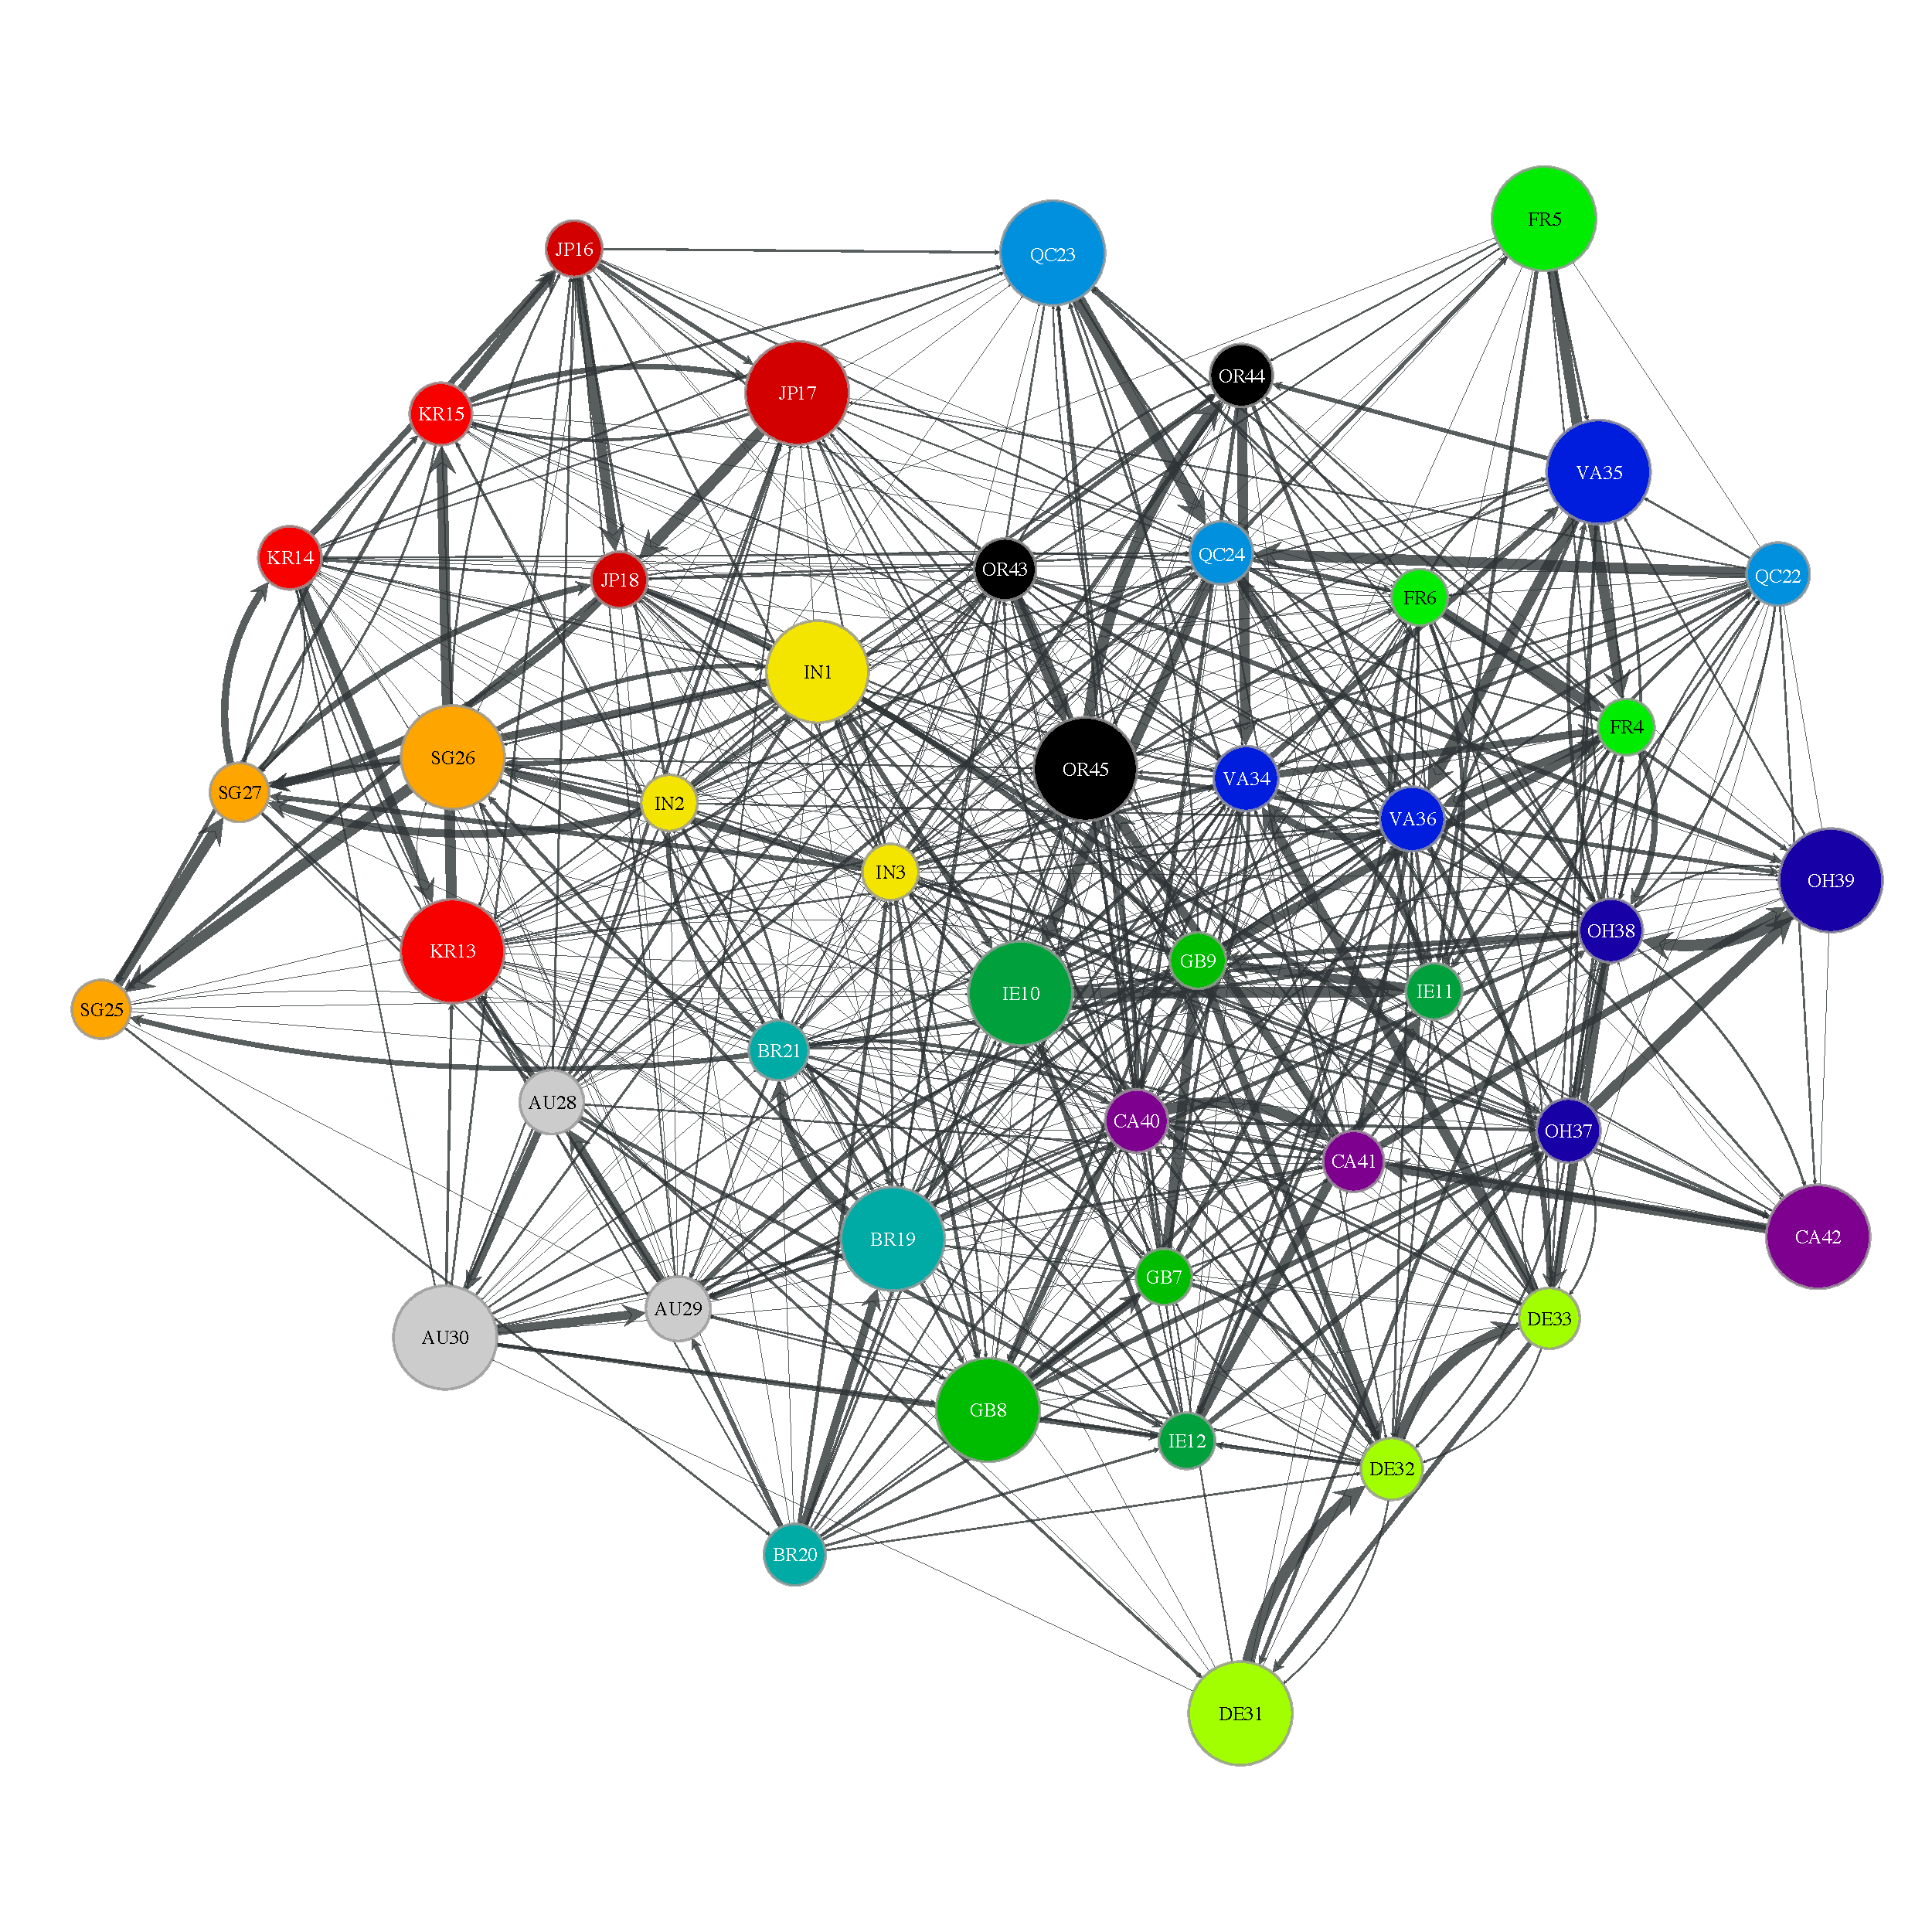
\includegraphics[width=5in]{figures/ch06_b-epsilon-greedy-0-2-e3.pdf}
    \end{center}
    \renewcommand{\baselinestretch}{1}
    \small\normalsize

    \begin{quote}
        \caption[Greedy Epsilon Anti-Entropy Synchronization Network]{Synchronization network using bandit based selection of synchronization peers with $\epsilon=0.2$.}
        \label{fig:ch06_epsilon_greedy_topology}
    \end{quote}
\end{figure}
\renewcommand{\baselinestretch}{2}
\small\normalsize

\begin{figure}
    \begin{center}
        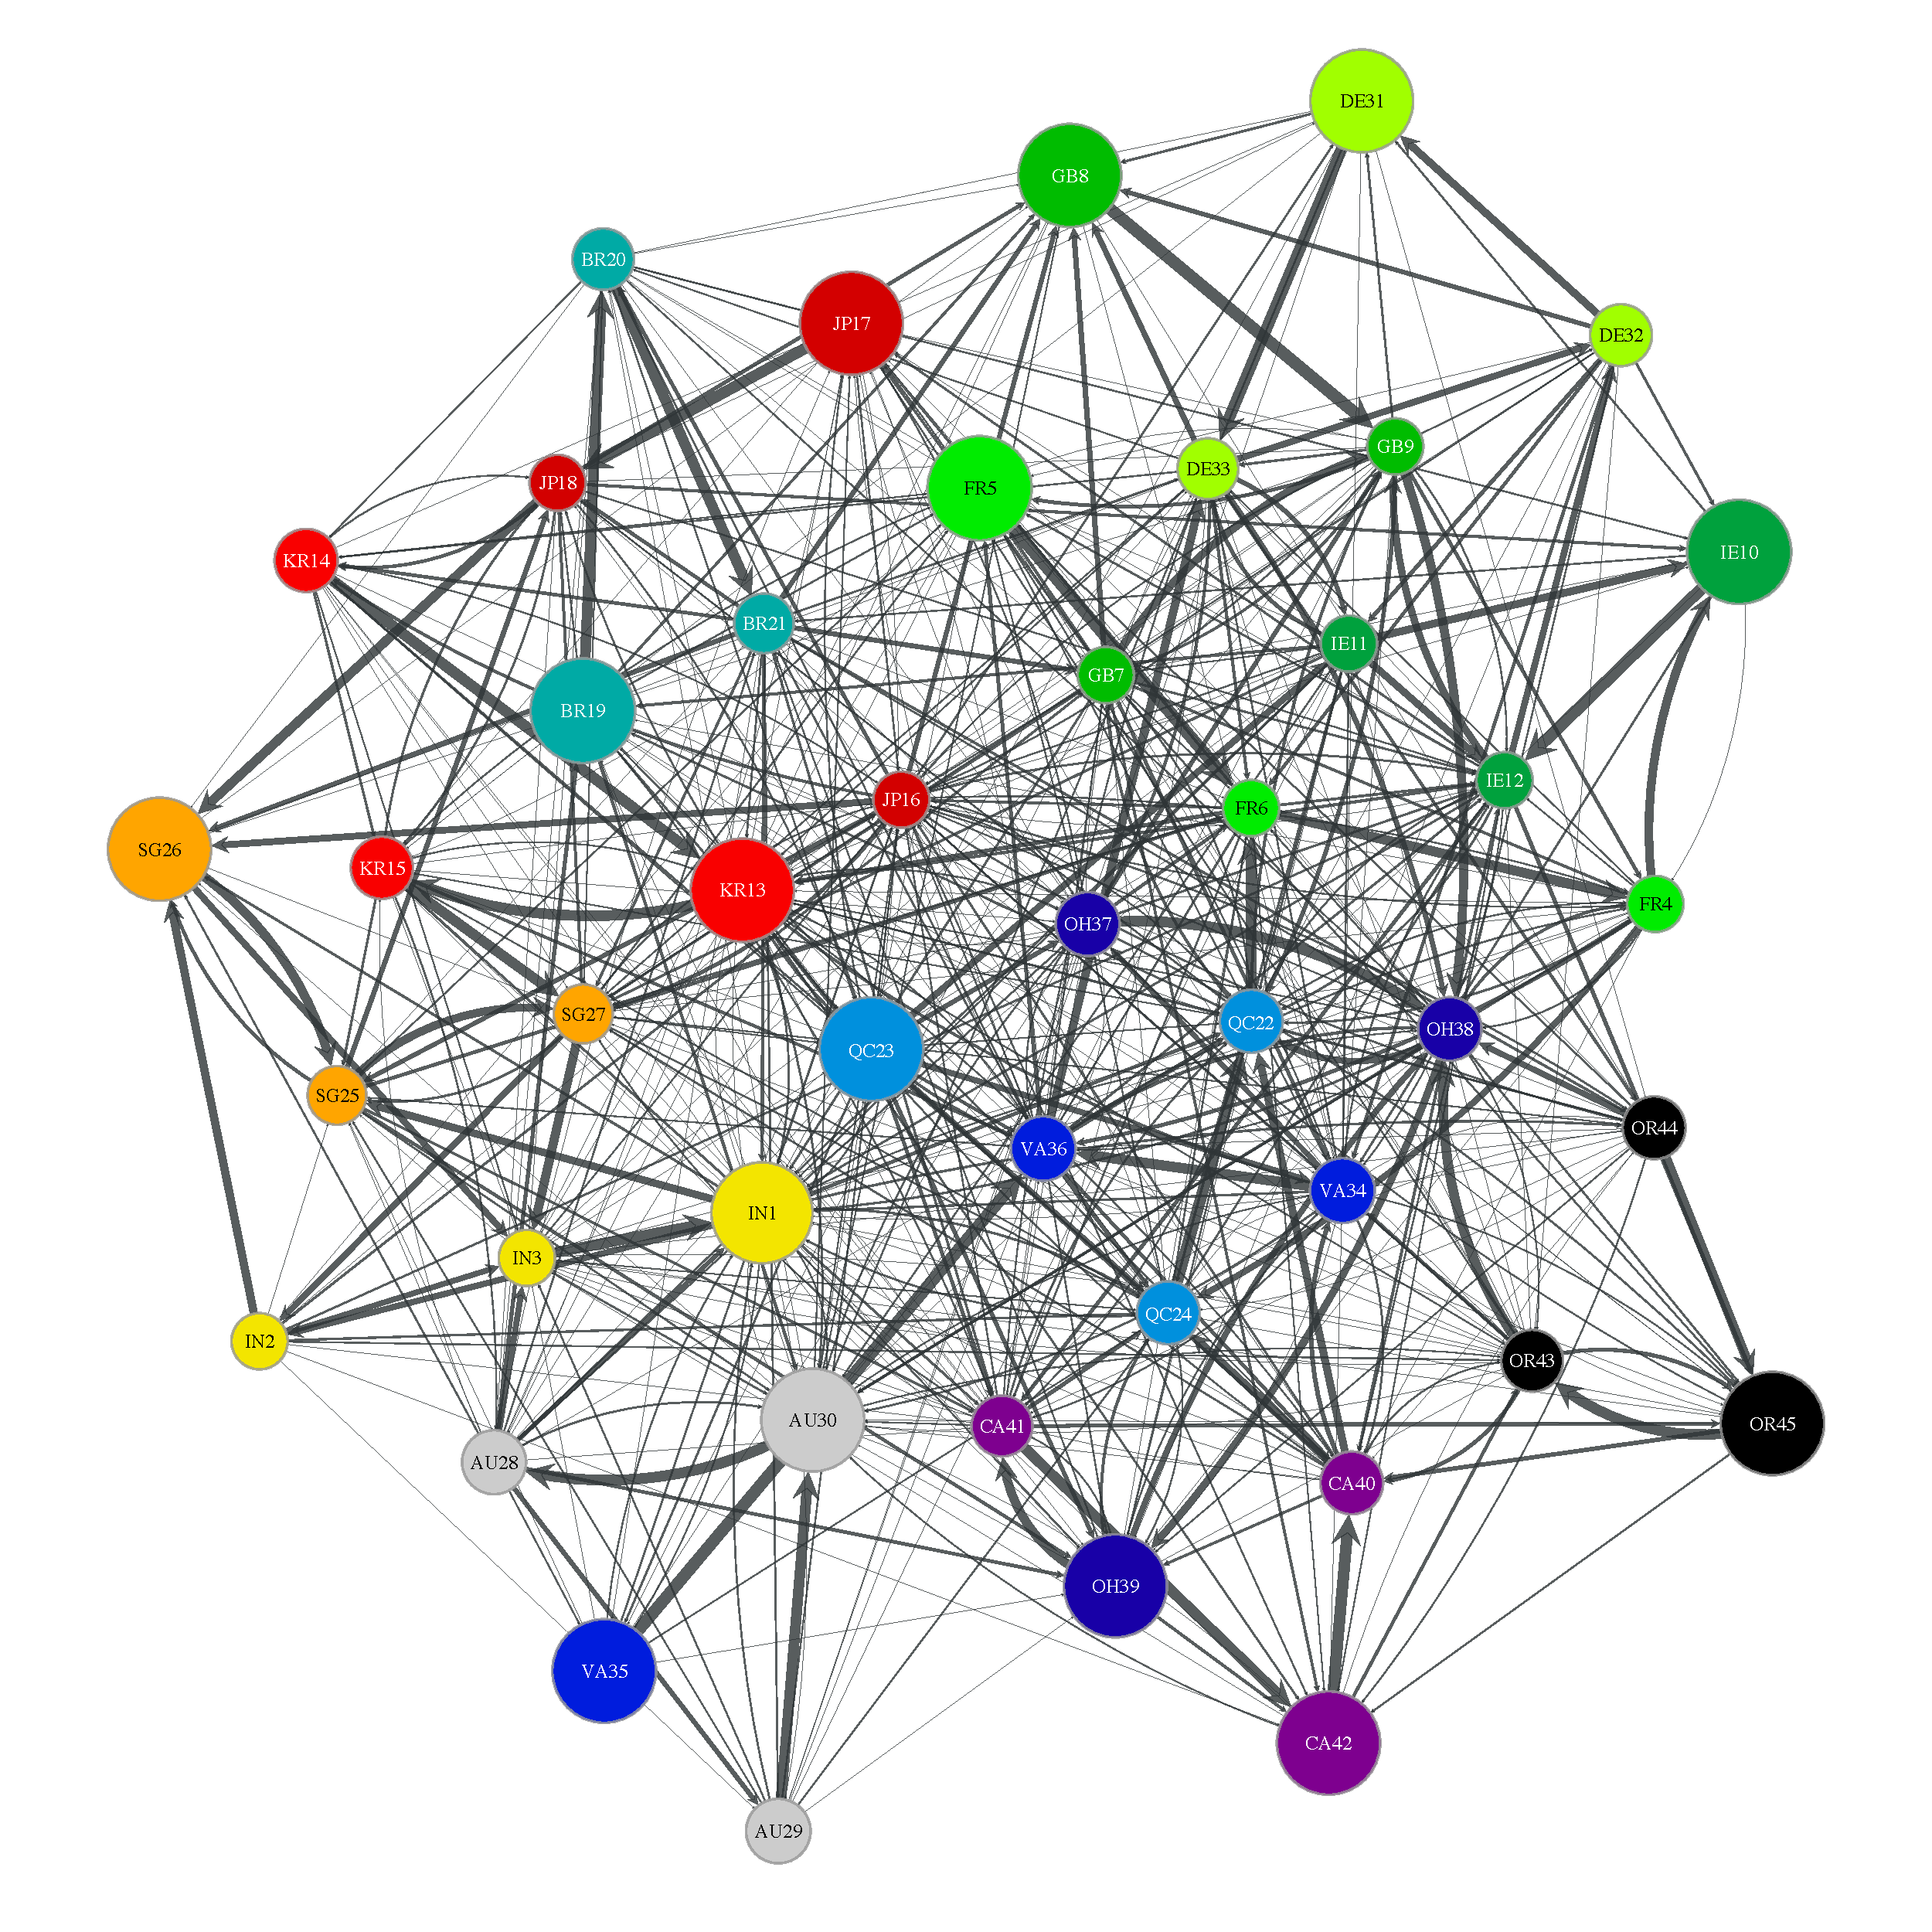
\includegraphics[width=5in]{figures/ch06_b-annealing-epsilon-greedy-e5.pdf}
    \end{center}
    \renewcommand{\baselinestretch}{1}
    \small\normalsize

    \begin{quote}
        \caption[Annealing Epsilon Anti-Entropy Synchronization Network]{Synchronization network using annealing epsilon bandit based selection of synchronization peers.}
        \label{fig:ch06_annealing_epsilon_toplogy}
    \end{quote}
\end{figure}
\renewcommand{\baselinestretch}{2}
\small\normalsize

Comparing the resulting networks, it is easy to see that more defined
topologies result from the bandit-based approaches.
The uniform selection network is simply a hairball of connections with
a limited number of synchronizations.
Clear optimal connections have emerged with the bandit strategies, dark
lines represent extremely successful synchronization connections between
replicas, while light lines represent synchronization pairs that are
selected less frequently.
We posit that fewer edges in the graph represents a more stable network;
the fewer synchronization pairs that are selected, the less noise that
occurs from selecting a peer that is in a similar state.

\section{Bandits Discussion}

To achieve stronger eventual consistency, the visibility latency
of a system replicated with anti-entropy must be reduced.
We believe that this can be achieved with two primary goals: increasing
the number of successful synchronizations and maximizing the number
of local and regional synchronizations such that the average latency of
anti-entropy sessions is as low as possible.
These goals must also be tempered against other requirements, such as
fault and partition tolerance, a deterministic anti-entropy solution that
ensures the system will become consistent eventually, and load balancing
the synchronization workload evenly across all replicas.

Bandit based approaches to peer selection clearly reduce noise inherent
in uniform random selection as shown in Figure~\ref{fig:ch06_rewards}.
The bandit strategies achieve better rewards over time because peers
are selected that are more likely to have an update to synchronize.
Moreover, based on the network diagrams shown in
Figures~\ref{fig:ch06_uniform_selection_topology}-\ref{fig:ch06_epsilon_greedy_topology}, this is
not the result of one or two replicas becoming primary syncs: most
replicas have only one or two dark in-edges meaning that most replicas
are only the most valuable peers for one or two other replicas.

Unfortunately, the rewards using a bandit approach, while clearly better
than the uniform case, are not significantly better -- this is an interesting
demonstration of the possibility of adaptive systems to improve consistency
but further investigation is required.
The primary place we see for adjustment is future work to explore the reward
function in detail.
For example, the inclusion of penalties (negative rewards) might make
the system faster to adjust to a high quality topology.
Comparing reward functions against variable workloads may also reveal a
continuum that can be tuned to the specific needs of the system.

As for localization, there does appear to be a natural inclination for
replicas that are geographically proximate to be a more likely selection.
In Figure~\ref{fig:ch06_epsilon_greedy_topology}, replicas in Canada (light blue),
Virginia (dark blue), Sydney (grey), California (purple), and Frankfurt
(light green) all prioritize local connections.
Regionally, this same figure shows strong links such as those between Ohio
and California (\texttt{CA42} $\rightarrow$ \texttt{OH38}) or Japan and
Singapore (\texttt{JP17} $\rightarrow$ \texttt{SG25}).
Replicas such as \texttt{BR19} and \texttt{IN3} appear to be hubs that
specialize in cross-region collaboration.
Unfortunately there does also seem to be an isolating effect, for example
Sydney (grey) appears to have no significant out of region synchronization
partners.
Isolated regions could probably be eliminated by scaling rewards with
the number of transmitted updates, or by using larger epsilons.
Multi-stage bandits might be used to create a tiered reward system to
specifically adjust the selection of local, regional, and global peers.
Other strategies such as upper confidence bounds, softmax, or Bayesian
selection may also create more robust localization.

Finally, and perhaps most significantly, the experiments conducted in
this paper were on a static workload; future work must explore dynamic
workloads with changing access patterns to more closely simulate real
world scenarios.
While bandit algorithms are considered online algorithms that do respond
to changing conditions, the epsilon greedy strategy can be slow to change
since it prefers to exploit high-value arms.
Contextual bandits use side information in addition to rewards to make
selection decisions, and there is current research in exploring contextual
bandits in dynamic worlds that may be applicable~\cite{contextual_bandits}.
Other strategies such as periodic reseting of the values may incur a small
cost to explore the best anti-entropy topology, but could respond to changing
access patterns or conditions in a meaningful way.

Future efforts will consider different reward functions, different selection
strategies, dynamic environments, and how the priorities of system designers
can be embedded into rewards.
Reward functions that capture more information about the expected workload of
the system such as object size, number of conflicts, or localizing objects
may allow specific tuning of the adaptive approach.
We will also specifically explore in detail the effect of dynamic workloads
on the system and how the reinforcement learning can adapt in real time to
changing conditions.
We plan to investigate periodic resets, anomaly detection, and auction
mechanisms to produce efficient topologies that are not brittle as access
patterns change.
We also plan to evaluate other reinforcement learning strategies such as
neural or Bayesian networks to determine if they handle dynamic environments
more effectively.

\section{Access Temperature Approaches}

\todo{add this section}

- Expected model of access patterns (daylight).

\section{Other Types of Adaptation}

\todo{add this section and conclusion}

Monitor and Optimize.

Replica placement, object placement


\section{Conclusion}

In this chapter we have presented a demonstration of adaptive consistency in
the geo-replicated eventually consistent systems by employing a novel
approach to peer selection during anti-entropy -- replacing uniform random
selection with multi-armed bandits.
Multi-armed bandits consider the historical reward obtained from
synchronization with a peer, defined by the number of objects synchronized
and the latency of RPCs, when making a selection.
Bandits balance the exploitation of a known high-value synchronization
peer with the exploration of possibly better peers or the impact of
failures or partitions.
The end result is a replication network that is less perturbed by noise
due to randomness and capable of more efficiently propagating updates.

In an eventually consistent system, efficient propagation of updates is
directly tied to higher consistency.
By reducing visibility latency, the likelihood of a stale read decreases,
which is the primary source of inconsistency in a highly available system.
We have demonstrated that bandit approaches do in fact lower visibility
latency in a large network.

We believe that the results presented show a promising start to a renewed
investigation of highly available distributed storage systems in novel
network environments, particularly those that span the globe.
Specifically, this work is part of a larger exploration of adaptive,
globally distributed data systems that federate consistency levels to provide
stronger guarantees~\cite{federated_consistency_poster}.
Federated consistency combines adaptive eventually consistent systems such as
the one presented in this paper with scaling geo-replicated consensus such as
Hierarchical Consensus~\cite{hc_brief_announcement} in order to create robust
data systems that are automatically tuned to provide the best availability
and consistency.
Distributed systems that adapt to and learn from their environments and
access patterns, such as the emerging synchronization topologies we observed
in this paper, may form the foundation for the extremely large, extremely
efficient networks of the future.
